\problemname{Tycho}

\illustration{.4}{img/MarsPerseveranceRover.jpg}{}

\noindent
% The planetary exploration vehicle \emph{Tycho VIII} needs to get back to 
% the home base after collecting mineral samples.
Planeetantutkimusmönkijän \emph{Tycho VIII}:n täytyy palata takaisin tukikohtaansa 
kerättyään mineraalinäytteitä.
% Tycho travels in a straight line from position~$0$ to the home base at position~$b$.
Tycho liikkuu suoralla viivalla pisteestä~$0$ tukikohtaan pisteessä~$b$.
% While moving, it advances at a slow but steady pace of $1$~unit per second.
Se liikkuu eteenpäin hitaalla mutta varmalla $1$~yksikön nopeudella.
% Every second, Tycho takes $1$~unit of environmental damage from the harsh 
% planetary conditions.
Joka sekunti Tycho ottaa $1$~yksikön ympäristövahinkoa planeetan ankarien 
olosuhteiden takia.

% The situation is made even worse by radiation from a nearby pulsar, which 
% adds $d$ additional units of damage every $p$ seconds.
Tilannetta pahentaa vielä lisää se, että läheisestä pulsarista tulee säteilyä, joka 
aiheuttaa $d$ yksikköä lisävahinkoa $p$:n sekunnin välein.
% However, the radiation damage can be avoided by seeking shelter in one of 
% $n$ different hiding spots---caves, vegetation, large rocks, carcasses of 
% the planet's megafauna---along the way.
Säteilyvahingon voi kuitenkin välttää etsimällä suojaa yhdestä $n$:stä eri 
piilopaikasta---luolista, kasvillisuudesta, suurista kivistä, planeetan megafaunan 
raadoista---matkan aikana.
% Tycho can choose to stand still at any point for any integer number of seconds.
Tycho voi valita pysyä paikallaan missä tahansa kokonaislukumäärän sekunteja.

% The starting position~$0$ and the home base at~$b$ are both sheltered, so 
% Tycho takes no radiation damage there.
Sekä alkupiste~$0$ että tukikohta~$b$ ovat suojattuja, joten Tycho ei saa 
säteilyvahinkoa niissä ollessaan.

\medskip
% What is the minumum damage Tycho will take on its journey back to the home base?
Mikä on pienin määrä vahinkoa, jonka Tycho voi saada matkallaan tukikohtaan?

\section*{Esimerkki}

% Consider the situation where the home base is at position $18$ and there 
% are shelters at positions $8$ and $15$.
Tarkastellaan tilannetta, jossa tukikohta on kohdassa $18$ ja suojia on kohdissa $8$ ja $15$.

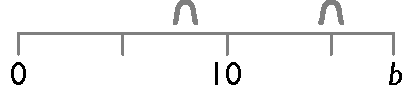
\includegraphics[width=.3\textwidth]{img/samplesetup}

% Assume that the pulsar's period is $4$, so unsheltered Tycho would take 
% damage at times $4$, $8$, $12$, etc.
Oletetaan, että pulsarin jaksonaika on $4$, eli suojaamaton Tycho saisi vahinkoa 
hetkillä $4$, $8$, $12$, jne.
% If Tycho leaves from the starting position (where it's sheltered) at time 
% $0$, it can reach the first shelter after $8$ seconds, incurring radiation 
% damage $d$ at time $4$ (but none at time $8$ because it's sheltered then).
Jos Tycho lähtee alkupisteestä (jossa se on suojassa) hekellä $0$, niin se 
voi saavuttaa ensimmäisen suojan $8$ sekunnissa, kerryttäen $d$ yksikköä säteilyvahinkoa 
hetkellä $4$ (mutta ei yhtään hetkellä $8$ koska se on silloin suojassa).
% Continuing without stopping, it reaches the home base at time $18$, incurring 
% $d+d$ more units of radiation damage (at times $12$ and $16$, respectively).
Jatkaen pysähtymättä, se saavuttaa tukikohdan hetkellä $18$, kerryttäen $d+d$ 
yksikköä lisää säteilyvahinkoa (hetkillä $12$ ja $16$). 
% This way it incurs $d+d+d=3d$ units of radiation damage and $18$ units of 
% environmental damage.
Tällä tavoin se kerryttää $d+d+d=3d$ yksikköä säteilyvahinkoa ja $18$ yksikköä 
ympäristövahinkoa.
% If instead Tycho waits at the $2$nd shelter (at position $15$) for $1$ 
% second, the pulse at time $16$ causes it no damage, and it reaches the 
% home base at time $19$ with a total of $2d + 19$ units of damage.
Jos taas Tycho odottaa $2.$ suojassa (kohdassa $15$) $1$ sekunnin, niin 
hetken $16$ pulssi ei aiheuta sille vahinkoa, vaan se pääsee tukikohtaan 
hetkellä $19$ saaden yhteensä $2d + 19$ yksikköä vahinkoa.
% This is better for most values of $d$.
Tämä on parempi suurimmalle osalle $d$:n mahdollisista arvoista.
% The two situations are shown here:
Nämä kaksi tilannetta on esitetty tässä:

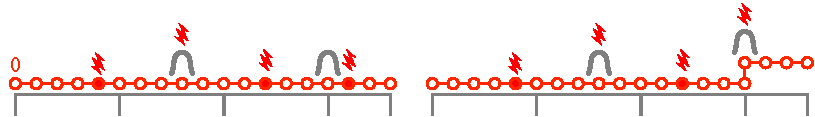
\includegraphics[width=.8\textwidth]{img/sample1_2.pdf}

% If the pulsar's period is $10$, Tycho can wait at the starting position 
% for $2$~seconds and then just go home without stopping at any shelter.
Jos pulsarin jaksonaika on $10$, niin Tycho voi odottaa alkupisteessä $2$~sekuntia 
ja sitten vain mennä tukikohtaan py\-säh\-ty\-mät\-tä mihinkään suojaan.
% Thus it passes the $1$st shelter (at position~$8$) at just the right 
% moment when the pulsar flares and arrives at the home base at time $20$, 
% for a total of $20$ environmental damage and no radiation damage at all.
Silloin se ohittaa $1.$ suojan (kohdassa~$8$) juuri oikealla hetkellä, 
kun pulsarin purkaus tapahtuu, ja saapuu tukikohtaan hetkellä $20$, 
saaden yhteensä $20$ ympäristövahinkoa eikä yhtään säteilyvahinkoa.

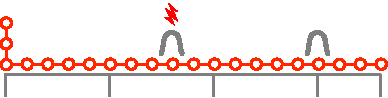
\includegraphics[width=.4\textwidth]{img/sample3.pdf}

\section*{Syöte}

% The first line consists of four integers $b$, $p$, $d$, and $n$, separated 
% by single spaces:
Syötteen ensimmäinen rivi sisältää neljä kokonaislukua $b$, $p$, $d$, ja $n$ 
välilyönneillä erotettuina:
% the location $b$ of the home base,
tukikohdan sijainti $b$,
% the pulsar's flare period~$p$,
pulsarin purkauksien jaksonaika~$p$,
% the additional radiation damage~$d$ caused by each flare of the pulsar,
pulsarin jokaisen purkauksen aiheuttama lisävahinko~$d$,
% the number~$n$ of the shelters.
suojapaikkojen määrä~$n$. 
% The following $n$~lines each contain an integer giving the shelter 
% locations $a_1$, $\ldots$, $a_n$, with 
% $0<a_1<\cdots <a_n< b$. % constraint:shelterbounds, constraint:sortedshelters
Seuraavat $n$~riviä sisältävät jokainen yhden kokonaisluvun, 
suojien sijainnit $a_1$, $\ldots$, $a_n$, missä 
$0<a_1<\cdots <a_n< b$. % constraint:shelterbounds, constraint:sortedshelters

\section*{Tuloste}

% Print a single integer: the minimum amount of damage Tycho must take 
% to reach $b$.
Tulosta yksi kokonaisluku: pienin määrä vahinkoa, joka Tychon täytyy saada 
päästäkseen $b$:hen. 


\section*{Rajoitukset ja pisteytys}

%You can assume
Voit olettaa, että
$p < b$ % constraint:pulsehappens
%and
ja 
$n < b$. % constraint:sheltersfit
%We always have
Kaikille syötteille pätee
$1\leq b\leq 10^{12}$, % constraint:b
$0\leq d \leq 10^6$, %constraint:d
%and
ja
$0\leq n \leq 10^5$. % constraint:n

% Your solution will be tested on a set of test groups, each worth a number of points.
Ratkaisu testataan testiryhmillä, joista kullakin on oma pistemäärä.
% Each test group contains a set of test cases.
Jokainen testiryhmä sisältää joukon testitapauksia.
% To get the points for a test group you need to solve all test cases in the test group.
Ryhmän pisteet saa vain, jos ratkaisee kaikki sen testitapaukset.
% Your final score will be the maximum score of a single submission.
Tehtävän lopullinen pistemäärä on suurin yksittäisen lähetyksen pistemäärä.


\medskip
\begin{tabular}{lll}
Ryhmä & Pisteet & Rajoitukset \\\hline
  $1$ & $8$  & $p\leq 10^6$ 
  % and Tycho does not need to wait \emph{after} 
  % leaving position
  ja Tychon ei tarvitse odottaa sen \emph{jälkeen} kun se on lähtenyt kohdasta~$0$.$^*$ \\ % constraint:nowait
  $2$ & $5$  & $b\leq 1000$, $p\leq 100$, $n\leq 10$ \\
  $3$ & $7$  & $b\leq 1000$ \\
  $4$ & $15$ & $p\leq 10^6$, $n\leq 1000$\\
  $5$ & $20$ & $p\leq 100$\\
  $6$ & $35$ & $p\leq 10^6$\\
  $7$ & $10$ & \emph{Ei muita rajoituksia}
\end{tabular}

\medskip
% \noindent $^*$ In test group~$1$, Tycho may still need to wait at 
% position~$0$ \emph{before} it starts moving.
% For example, sample inputs $2$, $3$, and $4$ belong to test group~$1$.
\noindent $^*$ Testiryhmässä~$1$ Tycho 
voi joutua odottamaan kohdassa~$0$ \emph{ennen} kuin se on alkanut liikkua.
Esimerkiksi e\-si\-merk\-ki\-syöt\-teet $2$, $3$, ja $4$ kuuluvat testiryhmään~$1$.
